\documentclass[11pt, oneside]{article} 
\usepackage{geometry}
\geometry{letterpaper} 
\usepackage{graphicx}
	
\usepackage{amssymb}
\usepackage{amsmath}
\usepackage{parskip}
\usepackage{color}
\usepackage{hyperref}

\graphicspath{{/Users/telliott/Github/figures/}}
% \begin{center} \includegraphics [scale=0.4] {gauss3.png} \end{center}

\title{Logarithms}
\date{}

\begin{document}
\maketitle
\Large

The logarithm and the exponential are inverse functions, we can see that if we plot them together:
\begin{center} 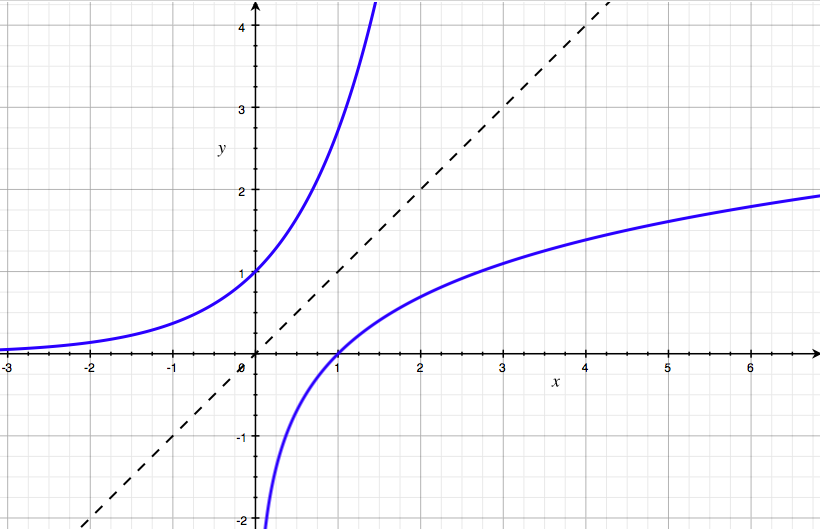
\includegraphics [scale=0.3] {log2.png} \end{center}
The upper curve is $y = e^x$ and the lower one is $y = \ln x$.
As inverse functions, they are symmetric about the line $y=x$.  

If we have that
\[ y = b^x \]
for some $b > 0, b \ne 1$, then we say that
\[ x = \log_b y \]

Putting them together
\[ y = b^{\ \log_b y} \]

The usual bases are 

$\circ$ \ $10$ (common logarithm, $\log_{10}$, or just $\log$)

$\circ$ \ $e$ (natural logarithm or $\ln$)

$\circ$ \ $2$ (binary logarithm, $\log_2$).

The rules for exponents are simple, if $p$ and $q$ are two numbers and we know the logarithms of $p$ and $q$ to base $b$
\[ p = b^{u} \]
\[ q = b^{v} \]
then their product can be computed as:

\[ pq = b^{u} \cdot b^{v} = b^{u + v} \]

To multiply two numbers, \emph{add} their logarithms.

It helps if we can actually compute $b^{u+v}$.  In the old days there were tables of logarithms, so you just looked up the answer in the table.

\begin{center} 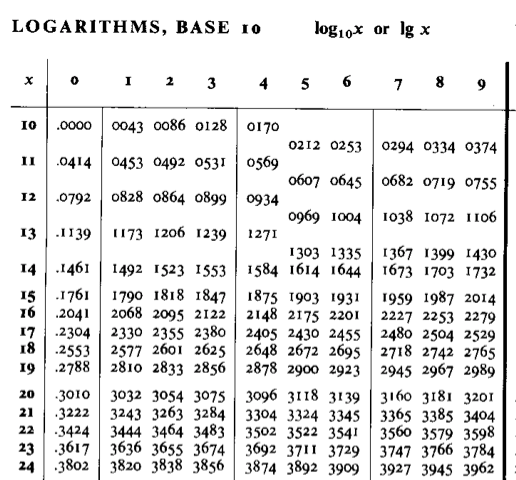
\includegraphics [scale=0.5] {log_table.png} \end{center}

$\log 2 \approx 0.3010$.

\url{https://en.wikipedia.org/wiki/Mathematical_table#Tables_of_logarithms}

The second rule is for exponentiation:
\[ (b^u)^v = b^{uv} \] 

And in terms of logarithms we can write
\[ uv = \log_b (b^u)^v \]
\[ = \log b^{uv} = v \log_b (b^u) \]

For example 
\[ 2^2 = 2 \cdot 2 = 4 \] 
\[ 2^3 = 2 \cdot 2 \cdot 2 = 8 \]
\[ 4 \cdot 8 = 2^2 \cdot 2^3 = 2^{2 + 3} = 2^5 \]
\[ = 2 \cdot  2 \cdot 2 \cdot 2 \cdot 2 = 32 \]
and
\[ (2^2)^3 = 4^3 = 64 = 2^6 = 2^{2 \cdot 3} \]

Here is a plot of $\log_{10}(x)$ and $\ln x$:
\begin{center} 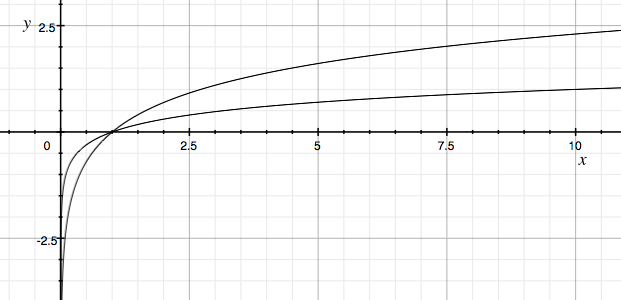
\includegraphics [scale=0.5] {log1.png} \end{center}
The first function reaches the value $1$ when $x=10$ and the second reaches the value $1$ when $x=e$.  Both have the value $0$ at $x=1$ because $b^0 = 1$ for any base, so the logarithm to any base of $1$ is equal to $0$.

It turns out that if we take the logarithm of $x$ (where $x$ is any number $> 1$) to two \emph{different} bases, the ratio of the logarithms is a constant, independent of the value of $x$.  And it is not hard to imagine that the ratios of the two values for any $x$ is a constant, in the plot above. 

\subsection*{change of bases}

This relationship is nicely shown by the change of bases formula.
\[ \log_b x = \frac{\log_a x}{\log_a b} \]

Derivation.

Start with an expression with $b$ as the base:
\[ y = b^x \]
and by the definition of the logarithm
\[ x = \log_b y \]

To derive the formula, take the logarithm to the base $a$ on both sides of the first expression:
\[ \log_a y = \log_a (b^x) \]

Now, just invoke the second rule on the right-hand side
\[ = x \log_a b \]
and then substitute for $x$ from the second expression above
\[ \log_a y = \log_b y \log_a b \]
We're basically done.

$\square$

$y$ can be any value, so replace it by $x$
\[ \log_a x = \log_b x \log_a b \]
Rearranging:
\[ \log_b x = \frac{\log_a x}{\log_a b} \]

Three ideas for remembering the formula.

(1) Learn the derivation.

(2) Logarithms of $x$ to different bases $b$ and $a$ are connected by some constant $k$
\[ \frac{\log_b x}{\log_a x} = k \]
\[ \log_b x = k \log_a x \]

and we substitute for $k$ the inverse of the log to the \emph{same} base as we have in the numerator:
\[ \log_b x = \frac{1}{\log_a b} \cdot \log_a x \]
that is, I remember that we want $\log_a$ something \emph{over }$\log_a$ something on the right. 

(3) You might look at the other formula
\[ \log_a x = \log_a b \log_b x  \]
and imagine the $b$'s canceling in some way.

One other thing we can do is to set $x=a$ in the above formula.  We start from
\[ \log_b x = \frac{\log_a x}{\log_a b} \]
then with $x=a$
\[ \log_b a = \frac{\log_a a}{\log_a b} \]
but $\log_a a = 1$ so
\[ \log_b a = \frac{1}{\log_a b} \]

And that makes perfect sense.  If we multiply by some factor $k$ to convert from the logarithm in base $a$ to base $b$, we must multiply by the inverse of the same factor to convert back again.

For the figure above of the common log (base 10) and the natural logarithm, $\ln 10 = 2.303$, and that looks about right, when $x=10$ the first function is $1.0$ and the second one is about $2.3$.

\subsection*{fractional exponents}
The introduction above dealt mainly with integer exponents, but of course you know that the practical use of logarithms depends on fractional values.  The simplest way to see how this works is to consider the square root.

\[ \sqrt{2} \times \sqrt{2} = 2 \]
If we think about what the exponent $u$ to the base $2$ would be such that
\[ 2^u = \sqrt{2} \]
We observe that by the rules for exponents
\[ \sqrt{2} \times \sqrt{2} = 2^u \times 2^u = 2^{u+u} = 2^1 \]

That is
\[ u + u = 1 \]
so $u = 1/2$.  By the same logic the $n^{\text{th}}$ root of $b$ is $b^{1/n}$.  And of course 
\[ (b^2)^{1/2} = b^{2 \times 1/2} = b^1 \]

\subsection*{fractional exponents}

Feynman has a nice description of how logarithms were calculated (see Lectures, volume 1, Chapter 22, Algebra)

\url{http://www.feynmanlectures.caltech.edu/I_22.html}

The basic idea is to take repeated square roots of the base ($10$), and then combine those to form the required value.

So for example
\[ 10^{1/2} = 3.1622776602 \]
this has been rounded up, the next term in the expansion is $3.162277 \dots$.  To obtain $10^{1/4}$, compute the square root of $10^{1/2}$.

\[ 10^{1/4} = 1.7782794100 \]
\[ 10^{1/8} = 1.3335214321 \]
\[ 10^{1/16} = 1.1547819847 \]
\[ 10^{1/32} = 1.07460782832 \]
\[ 10^{1/64} = 1.03663292844 \]
\[ 10^{1/128} = 1.0181517217 \]
\[ 10^{1/256} = 1.009035044841 \]
\[ 10^{1/512} = 1.004507364254 \]
\[ 10^{1/1024} = 1.002251148293 \]

and so on.  Eventually (around $10^{1024}$) we stop, because there is a neat trick that saves us from calculating.  It's a result from basic calculus so we won't say more.

Having these powers of $10$, now we want to compute a logarithm, say $\log_{10} 2$.  The first thing is that $2$ is smaller than $10^{1/2}$.  

So we start with 
\[ 2 = 10^{1/4} \cdot \ ?? \]

By trying the various powers of $10$, we settle on 
\[ 2 = 10^{1/4} \cdot 10^{1/32} \cdot 10^{1/64} \cdot 10^{1/256} \cdot r \]

We won't worry about the $r$, it is very close to $1$.

To get the logarithm of $2$ just add the logs of those powers:
\[ \log_{10} 2 = 0.25 + 0.03125 + 0.015625 + 0.00390625  = 0.30078125 \]

The actual value is 0.30103, to five places.

You can see that to get good accuracy, we will need to figure out the correction term.

\subsection*{Less than 1}
Fractional exponents leads to consideration of $0 < x < 1$.  Write
\[ x \cdot \frac{1}{x} = 1 \]
Take the logarithm of both sides
\[ \log(x \cdot \frac{1}{x} ) = \log 1 = 0 \]
\[ = \log x + \log \frac{1}{x} \]
Thus
\[ \log \frac{1}{x} = - \log x \]

\end{document}